\documentclass{beamer}

\mode<presentation> {
\usetheme{Madrid}
}

\usepackage{graphicx} % Allows including images
\usepackage{booktabs} % Allows the use of \toprule, \midrule and \bottomrule in tables
\usepackage{hyperref}
\usepackage{color}

\newcommand{\ut}[1]{\ensuremath{\tilde{#1}}}

%----------------------------------------------------------------------------------------
%	TITLE PAGE
%----------------------------------------------------------------------------------------

\title[Recycle Robot]{Motion Planning for Recycling Robotics: Progress Report} % The short title appears at the bottom of every slide, the full title is only on the title page

\author[Link, Tormey, LeVan]{Nicholas Link, Samuel Tormey, Ricky LeVan} % Your name

\date{\today} % Date, can be changed to a custom date

\begin{document}

\begin{frame}
\titlepage % Print the title page as the first slide

\end{frame}

\begin{frame}
\frametitle{Intro}
\begin{itemize}
\item We are building a simulated robot to manipulate objects on a conveyor belt
\item The desire to improve recycling efficiency inspired our project
\end{itemize}
\begin{centering}
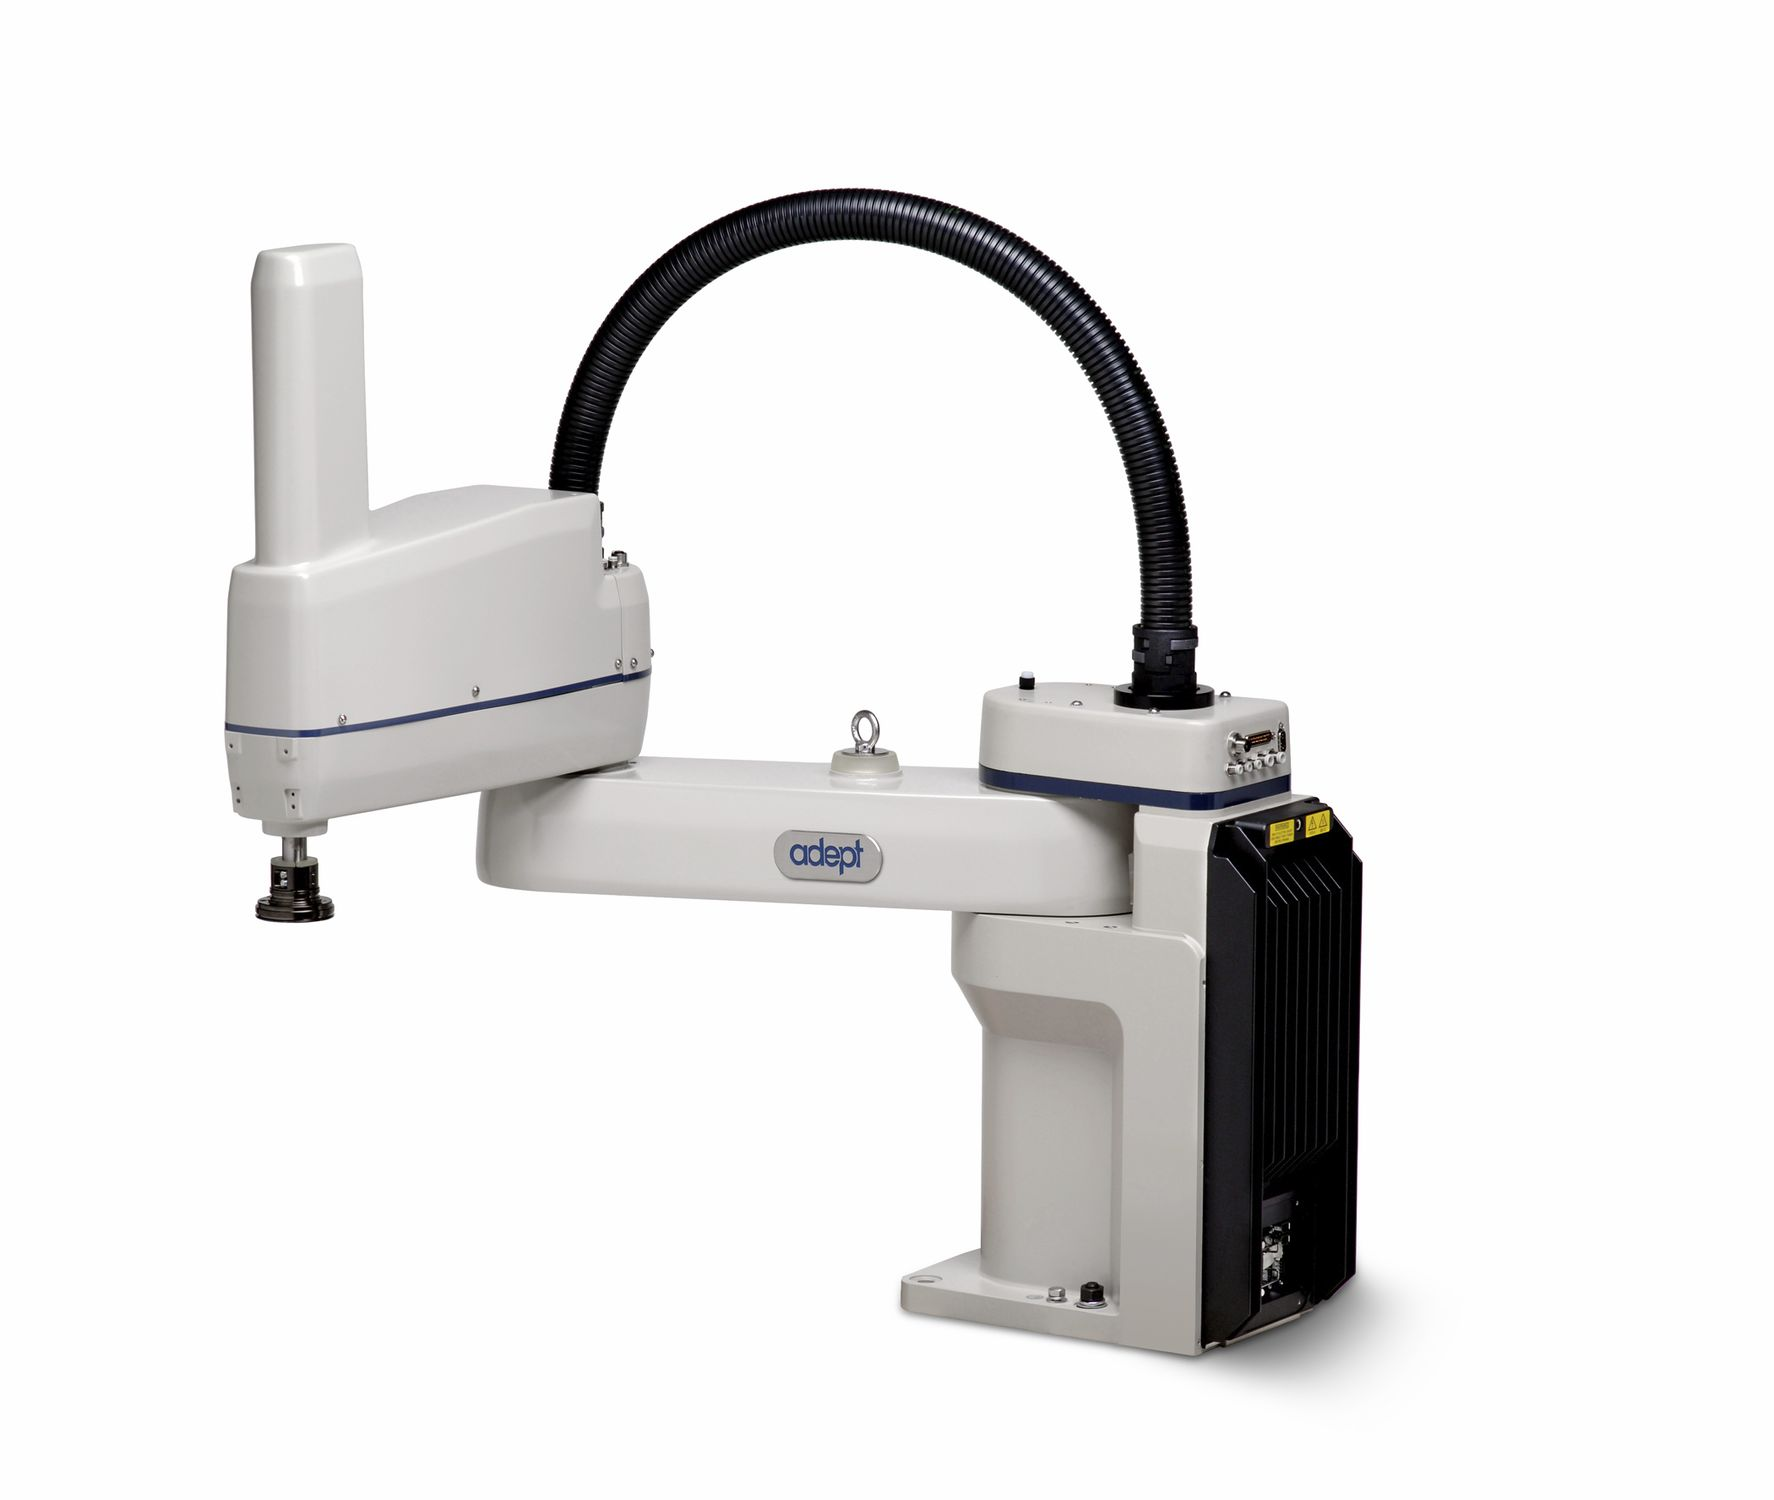
\includegraphics[width=0.55\linewidth,height=0.55\textheight,keepaspectratio]{/Users/nicklink/Documents/RecycleRobot/presentations/MidYearReport/scara.jpg}
%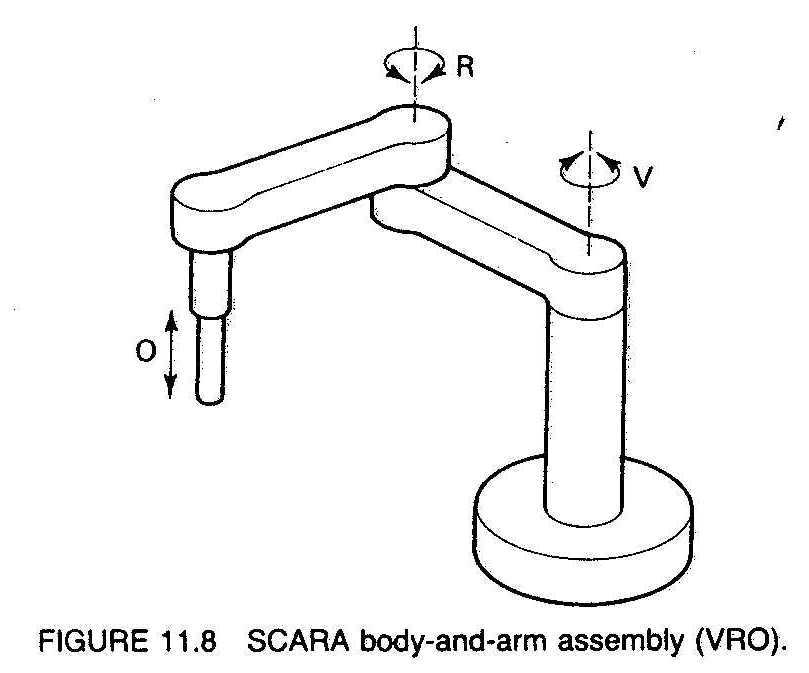
\includegraphics[width=0.55\linewidth,height=0.55\textheight,keepaspectratio]{scara2.jpg}
\end{centering}

\end{frame}


\begin{frame}
\frametitle{Review: Last Semester's Work}
\begin{itemize}
\item The core CAAM in our project comes from optimization
\item Last semester we studied the math behind this optimization
\item Comes in two kinds: optimizing path and optimizing picking strategy
\end{itemize}


\end{frame}


\begin{frame}
\frametitle{Current Progress Outline}
\begin{itemize}
\item Custom Jacobian
\item Initial guess optimizations
\item 3D robot animation
\end{itemize}

\end{frame}

\begin{frame}
\frametitle{Custom Jacobian}
Reminder: Our dynamics can be written in the following form:
$$b = \frac{x_{i+1} - x_i}{d\tau} - Tf(x_i,u_i) = 0$$

\end{frame}




\begin{frame}
\frametitle{Initial Guess Optimization}

\end{frame}


\begin{frame}
\frametitle{3-D Robot Animation}

\end{frame}


\begin{frame}
\frametitle{Semester Goals Outline}
\begin{itemize}
\item Online optimal path finding
\item Moving conveyor belt
\item Temporal goal planning
\end{itemize}

\end{frame}


\begin{frame}
\frametitle{Online performance}

\end{frame}


\begin{frame}
\frametitle{Moving Conveyor Belt}

\end{frame}


\begin{frame}
\frametitle{Temporal Goal Planning}

\end{frame}

\begin{frame}
\frametitle{End}

\end{frame}








\end{document}

